\begin{frame}[allowframebreaks]{Autoregressive Models: Modern Models}
    Modern autoregressive models have evolved significantly, leveraging advancements in neural network architectures and training techniques. Key developments include:

    \begin{itemize}
        \item \textbf{PixelCNN/PixelSNAIL:} Introduced convolutional layers to capture spatial dependencies in images, allowing for efficient pixel-wise generation.
        \item \textbf{WaveNet:} Applied dilated convolutions to model long-range dependencies in audio signals, achieving state-of-the-art results in speech synthesis.
        \item \textbf{Transformer-based Models:} Utilized self-attention mechanisms to capture global dependencies, enabling parallel processing and improved scalability.
    \end{itemize}

    These modern models have set new benchmarks in various domains, including image generation, speech synthesis, and text modeling.
    
    \framebreak
    
    \textbf{PixelCNN/PixelSNAIL:}
    \begin{itemize}
        \item Introduced by van den Oord et al. (2016) and later extended by Chen et al. (2017).
        \item Uses convolutional layers to model pixel dependencies in images.
        \item Each pixel is generated conditioned on previously generated pixels, allowing for efficient sampling.
        \item PixelCNN uses masked convolutions to ensure that each pixel is only influenced by previously generated pixels.
        \item PixelSNAIL extends this by incorporating self-attention mechanisms, allowing for better long-range dependencies.
    \end{itemize}
    
    \framebreak
    
    \textbf{WaveNet:}
    \begin{itemize}
        \item Introduced by van den Oord et al. (2016) for audio generation.
        \item Utilizes dilated convolutions to capture long-range dependencies in audio signals.
        \item Each audio sample is generated conditioned on previous samples, allowing for high-quality audio synthesis.
        \item Achieved state-of-the-art results in speech synthesis and music generation tasks.
    \end{itemize}
    \framebreak
    \textbf{Transformer-based Models:}
    \begin{itemize}
        \item Introduced by Vaswani et al. (2017) for natural language processing.
        \item Utilizes self-attention mechanisms to capture global dependencies in sequences.
        \item Allows for parallel processing, making it highly scalable for large datasets.
        \item Models like GPT-3 and BERT have set new benchmarks in various NLP tasks.
        \item Can be adapted for autoregressive generation tasks in images, audio, and other modalities.
    \end{itemize}
    \framebreak
    \textbf{Applications:}
    \begin{itemize}
        \item Image generation (e.g., PixelCNN, PixelSNAIL).
        \item Audio synthesis (e.g., WaveNet).
        \item Text generation and language modeling (e.g., Transformer-based models).
        \item Video generation and other multimodal tasks.
    \end{itemize}
    \framebreak
    \textbf{Pros:}
    \begin{itemize}
        \item High-quality generation across various modalities.
        \item Ability to capture complex dependencies in data.
        \item Scalability and efficiency in training and inference.
    \end{itemize}
    \textbf{Cons:}
    \begin{itemize}
        \item Computationally intensive, especially for large models.
        \item Requires large amounts of training data for optimal performance.
        \item Still faces challenges in handling very high-dimensional data efficiently.
    \end{itemize}
\end{frame}
\begin{frame}[allowframebreaks]{PixelCNN}
\textbf{Masked Spatial (2D) Convolution - PixelCNN}
\begin{itemize}
    \item Images can be flattened into 1D vectors, but they are fundamentally 2D.
    \item We can use a masked variant of ConvNet to exploit this knowledge.
    \item First, we impose an autoregressive ordering on 2D images:
\end{itemize}

\begin{figure}
    \centering
    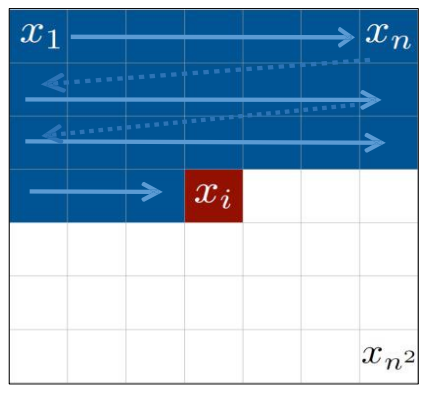
\includegraphics[height=0.4\textheight, width=\textwidth,keepaspectratio]{images/autoregressive/raster-scan.png}
    \caption*{Raster scan ordering of a 2D image. The pixels are processed in a left-to-right, top-to-bottom manner, similar to reading text.}
\end{figure}

\framebreak
\begin{itemize}
    \item The autoregressive ordering allows us to use a convolutional neural network (CNN) to predict the next pixel based on the previously generated pixels.
    \item We use masked convolutions to ensure that the model only has access to the pixels that have already been generated.
    \item The convolutional layers are designed to respect the autoregressive ordering, meaning that each pixel is predicted based on its left and top neighbours, but not the right or bottom neighbours.
\end{itemize}
\framebreak
\textbf{PixelCNNs}: Use the neighbour pixels to predict the new pixel.
\begin{columns}
        \begin{column}{0.5\textwidth}
            \begin{figure}
                \centering
                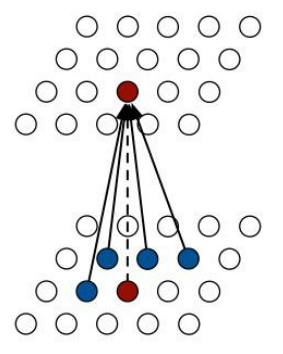
\includegraphics[width=0.9\textwidth, keepaspectratio]{images/autoregressive/pixelcnn.png}
                \caption*{Image generation with pixelCNN}
            \end{figure}
        \end{column}
        \begin{column}{0.5\textwidth}
            \begin{figure}
                \centering
                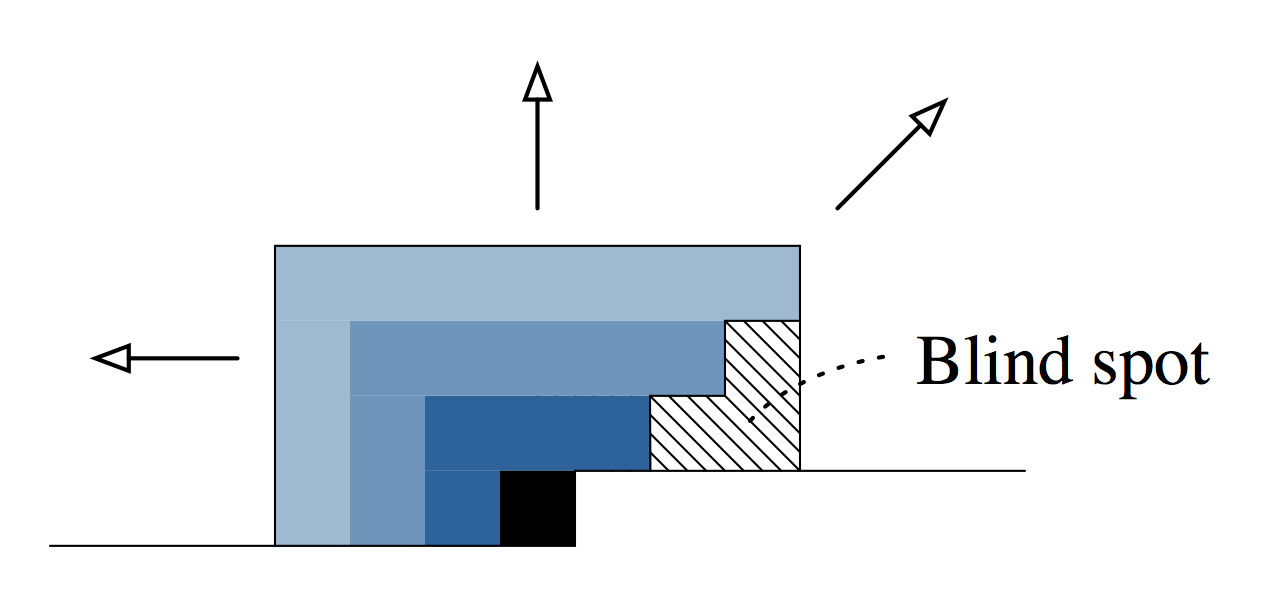
\includegraphics[width=1.1\textwidth,keepaspectratio]{images/autoregressive/pixelcnn-blindspot.png}
                \caption*{PixelCNN-style masking has one problem: blind spot in receptive field. The model cannot see the pixels to the right and below the current pixel, which can lead to artifacts in generated images.}
            \end{figure}
        \end{column}
    \end{columns}

\framebreak

\begin{itemize}
    \item PixelCNN results
        \begin{figure}
        \centering
        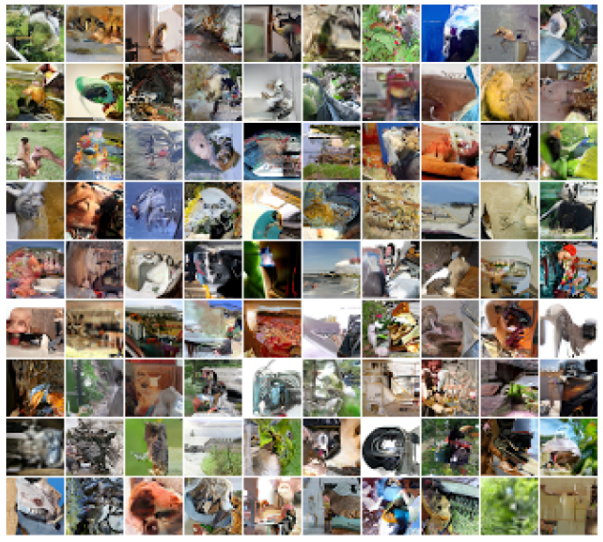
\includegraphics[height=0.65\textheight, width=\textwidth, keepaspectratio]{images/autoregressive/pixelcnn_results.png}
        \caption*{Image generation with pixelCNN. Model trained on Imagenet (32 x 32 pixels)}
    \end{figure}
\end{itemize}
\end{frame}